\documentclass[tikz,border=5mm]{standalone}
\usepackage{tikz}
\usetikzlibrary{matrix}

% --- COLOR DEFINITIONS ---
\definecolor{CGrayLight}{HTML}{E5E5E5}

\begin{document}
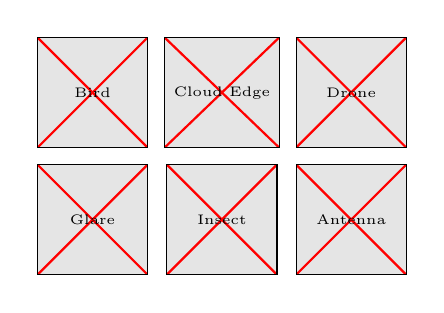
\begin{tikzpicture}[
    img/.style={draw, fill=CGrayLight, minimum size=1.4cm, font=\tiny, align=center},
    cross/.style={path picture={
      \draw[red, thick] (path picture bounding box.south west) -- (path picture bounding box.north east);
      \draw[red, thick] (path picture bounding box.north west) -- (path picture bounding box.south east);
    }}
]
  \matrix[row sep=2mm, column sep=2mm] {
    \node[img, cross] {Bird}; & \node[img, cross] {Cloud Edge}; & \node[img, cross] {Drone}; \\
    \node[img, cross] {Glare}; & \node[img, cross] {Insect}; & \node[img, cross] {Antenna}; \\
  };
\end{tikzpicture}
\end{document}
